\chapter{Introdução}
\label{sec:introducao}

Com o advento de novos recursos que podem ser provisionados sob demanda através da Internet, a chamada ‘nuvem’ envolve milhares de conexões entre servidores e usuários, provendo armazenamento, comunicações unificadas e alocação de recursos. Pessoas passaram a estar conectadas o tempo todo, com qualquer dispositivo que permita a troca de informações \cite{Seeber:2015}. As tecnologias atuais já não conseguem mais atender à todas as exigências dos usuários por causa de sua complexidade e quantidade de protocolos utilizados. Geralmente desenvolvidos e definidos de forma isolada e, para dificultar ainda mais, alguns fabricantes desenvolvem protocolos proprietários \cite{Kim:2013, Soares:2015}. Desta forma, a tarefa de alocar novos dispositivos para escalar a rede torna-se cada vez mais complexa e lenta, inviabilizando a implantação de novas tecnologias em uma rede já existente \cite{Kreutz:2014}. Essa inflexibilidade na arquitetura da Internet, traz um desafio para os pesquisadores da área, pois seus experimentos acabam não sendo validados em redes reais. 

O paradigma de Redes Definidas por Software, \gls{sdn}, e o protocolo OpenFlow \cite{OpenFlowSpec:2014} oferecem um caminho para vencer estes desafios, por meio de uma solução de implementação gradativa em redes de produção. O paradigma \gls{sdn} possibilita a rápida configuração de uma rede conforme a demanda de serviços, além de permitir adição de recursos, independente da fabricante \cite{Sayeed:2015}. A arquitetura \gls{sdn} provê uma abstração entre o plano de controle e o plano de dados, transformando \textit{switches} de rede em encaminhadores de pacote e a lógica, por sua vez, passa para controladores centralizados facilitando o gerenciamento da rede \cite{Kreutz:2013}. 

Para que essa abstração ocorra, é necessária uma comunicação entre os planos de controle e dados. Essa comunicação pode ser realizada através do protocolo OpenFlow, que atualmente vem sendo o protocolo mais utilizado em \gls{sdn} \cite{li:2016}. Em um \textit{switch} OpenFlow, há tabelas de fluxo (\textit{flow tables}) contendo regras para a manipulação de pacotes e estatísticas. Cada regra corresponde a um subconjunto do tráfego e para cada uma delas uma sequência de ações podem ser tomadas, como descarte, modificação do cabeçalho ou encaminhamento. Além disso são armazenadas estatísticas de cada fluxo recebido \cite{website:onf}.

\gls{sdn} provê uma visão global da rede, o que facilita o seu controle, porém a segurança continua sendo uma das principais preocupações na comunidade de rede devido ao abuso de recursos e intrusos maliciosos. Somente em 2016, foram reportadas 647.112 incidentes de segurança ao \gls{cert.br} \cite{certbr}, responsável por tratar incidentes de segurança e computadores que envolvam redes conectadas à Internet brasileira. Desse número, 59\% foram de ataques do tipo \textit{port scan}, ou em português, varredura de porta como pode ser visualizado na Figura \ref{fig:certbr}. Este alto número se deve basicamente por este tipo de ataque permitir a verificação de \textit{hosts} e serviços ativos na rede e que possam ser utilizados como porta de entrada para outros tipos de ataques.

\begin{figure}[H]
  \centering
  \caption{Incidentes Reportados ao \gls{cert.br} - Janeiro a Dezembro de 2016}
  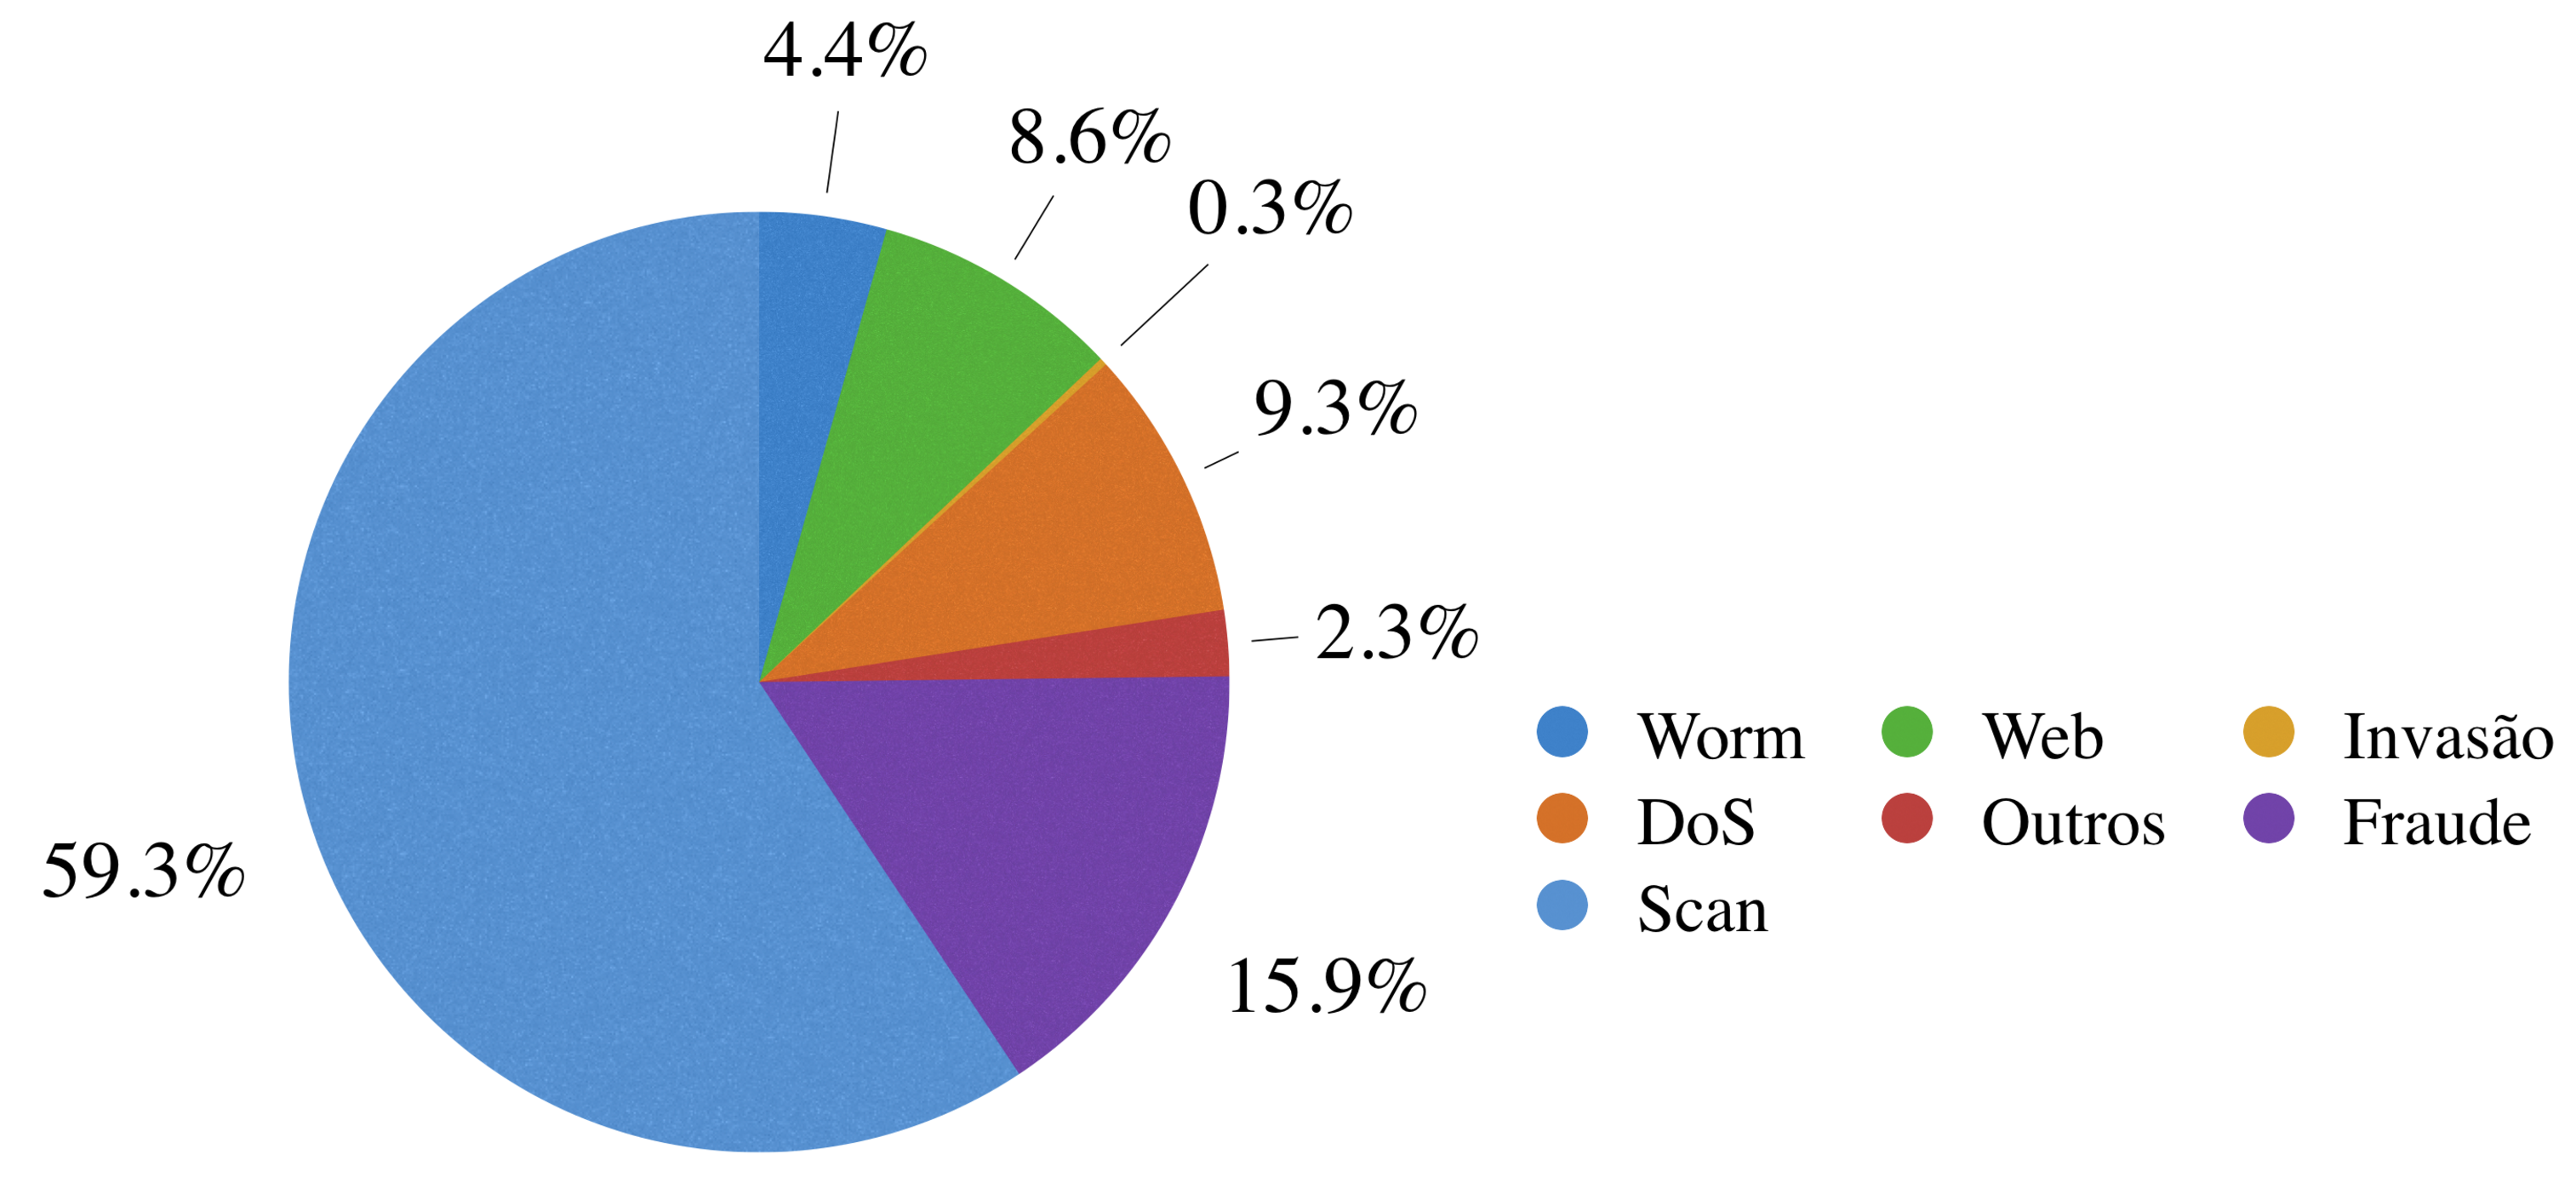
\includegraphics[width=.8\textwidth]{images/cert.eps}
  \label{fig:certbr}
  \fonte{Adaptado de \gls{cert.br}, 2017 \nocite{certbr}}
\end{figure}
\FloatBarrier

Tradicionalmente, Sistemas de Detecção de Intrusão, ou \textit{Intrusion Detection Systems} (IDS) \cite{Comer:2013}, são consideradas ferramentas comuns para detectar ataques maliciosos dentro de uma rede. Esses sistemas monitoram eventos de rede e tráfego para identificar atividades maliciosas e em seguida, emitir alertas e informar os administradores do sistema. 

A natureza de "detecção e alerta" das soluções de \gls{ids} atuais exige profissionais especialistas em segurança. Além disso, \glspl{ids} atuais carecem da atividade pró-ativa para evitar ataques em seu estágio inicial. Em um Sistema de Prevenção de Intrusão, \textit{Intrusion Prevention System} (IPS), essa tarefa de analisar e prevenir passa a ser realizada de forma automática, sem a necessidade de um profissional em segurança.

O \gls{ips} pode ser construído com base em um \gls{ids} pois a função de detecção é necessária em uma solução de \gls{ips}, contudo, a maioria das soluções existentes de \gls{ips} são desenhadas para a rede tradicional e uma simples migração para \gls{sdn} não é suficientemente eficaz para detectar e defender de ataques maliciosos \cite{Xiong:2014}.

Uma deficiência da maioria dos sistemas de detecção de intrusão é o fato de o seu funcionamento se basear na utilização de uma base de dados com assinatura de ataques: se um ataque conhecido é detectado, a tentativa é bloqueada, caso contrário, podem passar sem qualquer restrição. Essa análise também gera uma carga elevada a ser administrada caso a rede possua elevados índices de atividade, já que são verificados todos os pacotes que nela trafegam \cite{unifoa:2007}.

Uma maneira de contornar o problema da detecção por assinatura, é a utilização de sistemas de detecção que analisam o comportamento da rede. Neste, um modelo de normalidade é estabelecido em condições adequadas de uso (sem ataque), e comparado com a atividade em andamento. Qualquer comportamento suspeito, como aumento do tráfego ou pacotes incompletos, pode vir a ser considerado suspeito  \cite{unifoa:2007}.

Esta segunda técnica pode vir a reduzir a carga de administração por realizar a análise sobre uma amostra de pacotes, ou através da coleta de estatísticas disponíveis. Por outro lado, a detecção baseada em anomalia pode levar a alguns resultados não intuitivos, de forma a gerar um grande número de falsos positivos \cite{heberlein:2007}.

Observando as estatísticas de segurança e as soluções de \gls{ips} disponíveis para \gls{sdn}, foi discutido o seguinte problema: "É possível, através da coleta de estatísticas de tráfego, analisar, detectar e prevenir intrusões de forma eficaz em uma rede \gls{sdn}?". Em \gls{sdn}, através do protocolo Openflow, é possível a obtenção de estatísticas de tráfego de cada fluxo de dados diretamente dos comutadores, isso traz vantagens no que diz respeito a desempenho, pois não há a necessidade de sensores específicos. Além disso, a visão global de \gls{sdn} permite a proteção em tempo real de todo um sistema, enquanto que em redes tradicionais essa proteção é apenas local, uma vez protegido de um ataque, o fluxo poderá tomar outras rotas para atingir seu objetivo, problema que pode ser evitado facilmente em \gls{sdn}.

Com base no que foi discutido, este trabalho de conclusão apresenta uma metodologia de sistema de prevenção contra ataques de varredura de porta em \gls{sdn}. Para isso, utiliza como fonte de informações para análise de tráfego malicioso, os contadores das tabelas de fluxos de \textit{switches} OpenFlow, possibilitando assim, uma medida de detecção eficiente e proteção a nível global da rede.

O restante deste trabalho está dividido como segue. O Capítulo \ref{cap:fundamentacao} apresenta os conceitos necessários para o entendimento deste trabalho, descrevendo o funcionamento e arquitetura de \gls{sdn}, além de desafios no que diz respeito à segurança. O Capítulo \ref{cap:trabalhos-relacionados} apresenta algumas soluções \gls{ids}/\gls{ips} existentes na literatura bem como os objetivos deste. No Capítulo \ref{cap:metodologia} é apresentada a metodologia utilizada no desenvolvimento deste trabalho, detalhes de sua implementação e funcionamento. O ambiente utilizado para avaliação do \gls{ips} desenvolvido bem como os resultados obtidos são apresentados no Capítulo \ref{cap:testes} e, por fim, no Capítulo \ref{cap:consideracoes}, são descritas algumas considerações sobre este trabalho e para trabalhos futuros.